\newpage
\section{Results and Discussion} \label{sec:results}
The gathered measurements are shown in figure \ref{fig:measurements} (red dots), the calculated value (blue including the shaded uncertainty range) and the best fit (red dashed). The orange vertical line shows the range of the lock-in frequency.
\begin{figure}[h!]
    \centering
    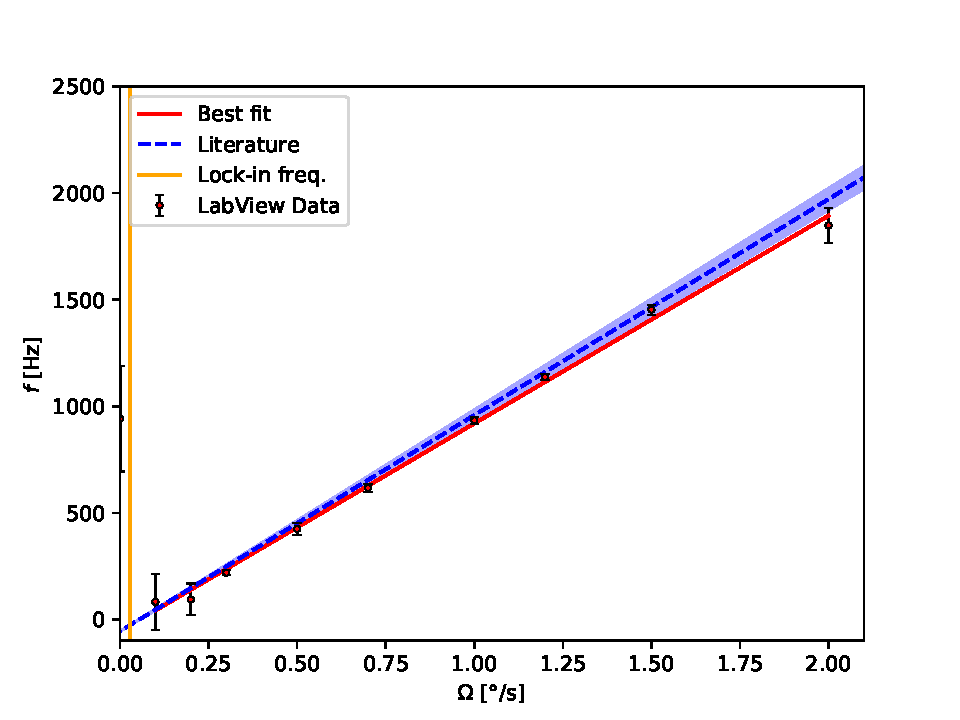
\includegraphics[width=\textwidth]{Gyroscope/Report/plots/slope_pos.pdf}
    \caption{The best fit applied only to the positive velocities.}
    \label{fig:measurements}
\end{figure}
dt = 1 ms on oscilloscope:
[1018.30201846  -86.64577303]
slope = (1018.30 +/- 16.28) krad/deg
offset = (-86.65 +/- 14.76) krad/s
\begin{figure}[h!]
    \centering
    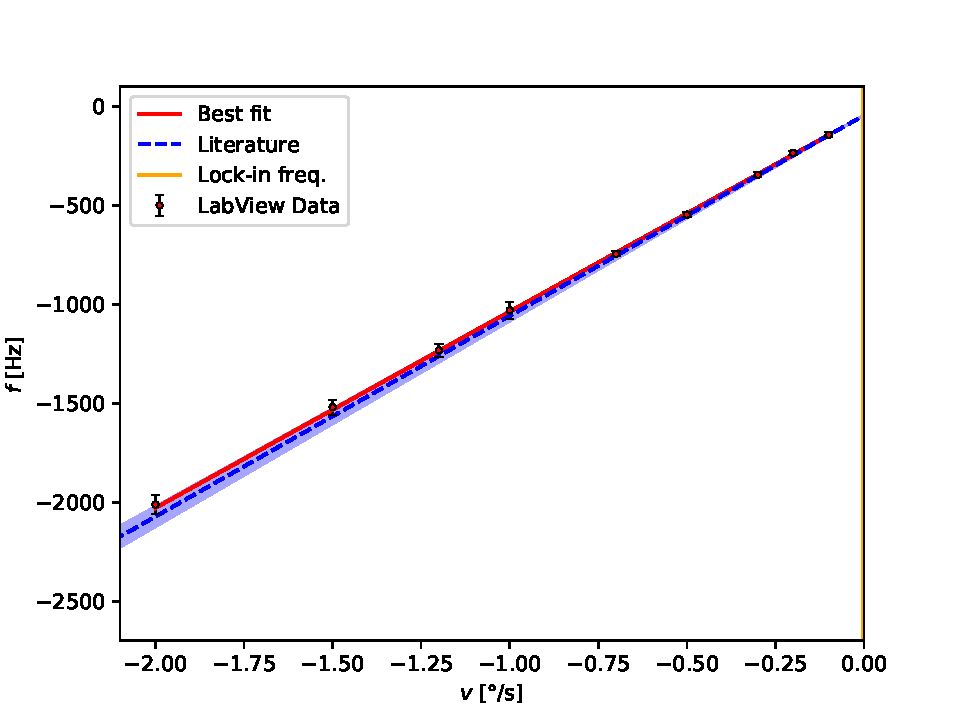
\includegraphics[width=\textwidth]{Gyroscope/Report/plots/slope_neg.pdf}
    \caption{The best fit applied only to the negative velocities.}
    \label{fig:measurements}
\end{figure}
dt = 1 ms on oscilloscope:
[991.66875925 -45.93399194]
slope = (991.67 +/- 14.88) krad/deg
offset = (-45.93 +/- 8.37) krad/s

\begin{figure}[h!]
    \centering
    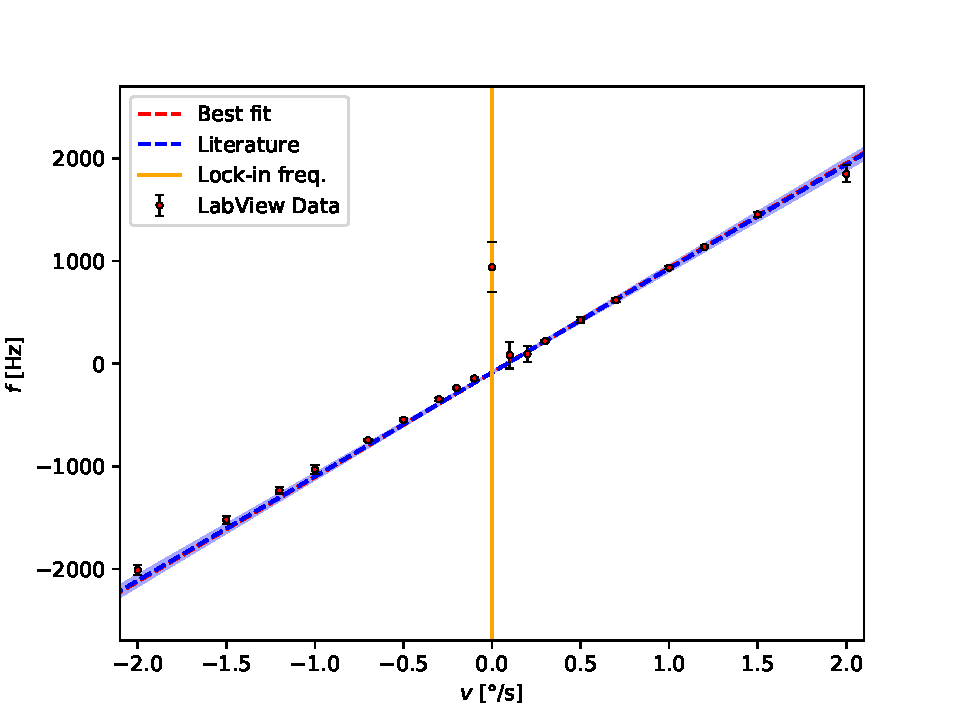
\includegraphics[width=\textwidth]{Gyroscope/Report/plots/slope.pdf}
    \caption{The best fit applied to all data-points.}
    \label{fig:measurements}
\end{figure}
The theoretically calculated value using equation \ref{eq:slope} is:
$$\Delta \nu = (1013.43 \pm 25.34)\, \Omega $$